\section{Applications}

\begin{frame}{Existing Applications}
Some existing applications of SPNs:
\begin{itemize}
    \item Computer vision, e.g.~image classification, medical image processing, attend-infer-repeat.
    \item Language processing, e.g.~language modelling, bandwidth extension.
    \item Robotics, e.g.~semantic mapping.
    \item \textbf{Non-linear regression}, and many more\footnote{\scriptsize https://github.com/arranger1044/awesome-spn\#applications}
\end{itemize}
\end{frame}

\begin{frame}{Gaussian Processes}
    A Gaussian Process (GP) is a collection of random variables indexed by an arbitrary
    covariate space $\mathcal{T}$, where any finite subset is Gaussian distributed.

    A GP can be understood as a prior over functions.

    \begin{figure}
        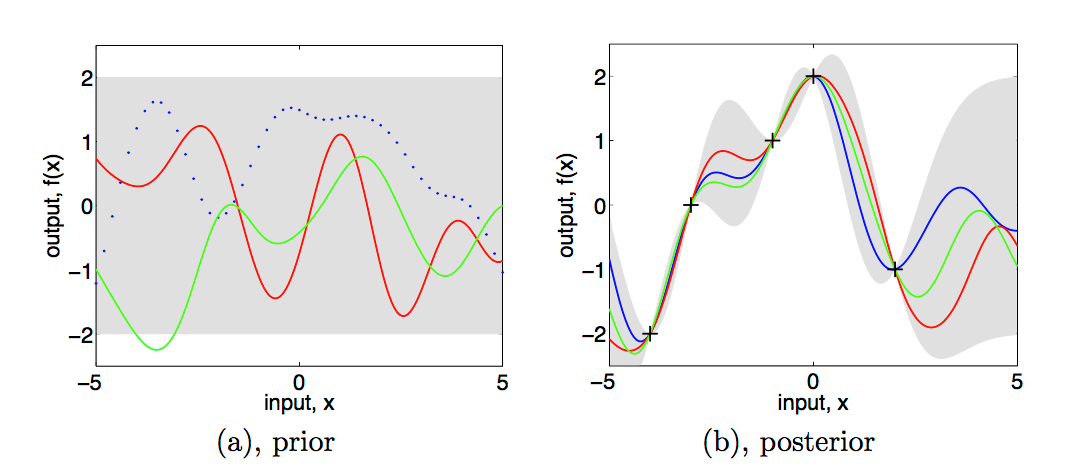
\includegraphics[width=0.9\textwidth]{GP_Rasmussen}
        \caption{\scriptsize C. E. Rasmussen \& C. K. I. Williams, Gaussian Processes for Machine Learning, 2006.}
    \end{figure}
\end{frame}

\begin{frame}{Gaussian Processes}
A GP is uniquely specified by a \emph{mean-function} $m: \mathcal{T} \rightarrow \mathbb{R}$ and a \emph{covariance function} $k: \mathcal{T} \times \mathcal{T} \rightarrow \mathbb{R}$.
%  \item Given a dataset $\data = \{(\x_n, y_n)\}_{n=1}^N$ with N observations where $f_n$ is the RV of observation $(\x_n, y_n)$, the joint distribution of the trainings data and a new datum $\xnew$ is Gaussian and the conditional of any Gaussian joint is again a Gaussian.

The posterior predictive distribution (used for predictions) of a GP is Gaussian, i.e.,
  \begin{equation}
    p(f^* \cbar \bm f) = \Normal\left( k^T_{\xnew,\X} k^{-1}_{\X,\X} \bm f , k_{\xnew,\xnew} - k_{\xnew,\X} k^{-1}_{\X,\X}k^T_{\xnew,\X}   \right)
  \end{equation}
\textbf{Problem:} How to compute the inversion of $k_{\X,\X}$?
%\end{itemize}
\end{frame}


\begin{frame}{Gaussian Processes}
We can use the Cholesky decomposition. % of $k_{\X,\X} = LL^T$ and take $(L^{-1})^T L^{-1}$ instead of $k^{-1}_{\X,\X}$.

\textbf{Problem:} The Cholesky decomposition scales $\mathcal{O}(N^3)$.

Solutions:
\begin{enumerate}
  \item Approximate the posterior using a variational approximation, or
  \item Use local experts to approximate the GP or approximate the computation of predictions.
\end{enumerate}
\end{frame}
%\iffalse

\begin{frame}{Local Experts}
\textit{Local experts to approximate the GP or approximate the computation of predictions.}

A natural way is to partition $\mathcal{T}$ into sub-sets $\mathcal{T}^{(k)} \; , k=1, \dots, K$. This is called the naive-local-experts model.
\begin{figure}
  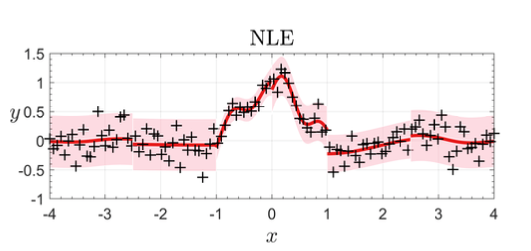
\includegraphics[width=0.8\textwidth]{NLE}
\end{figure}
\end{frame}


\begin{frame}{Local Experts}
Existing solutions to discontinuities.
\begin{enumerate}
    \item Product-of-Experts (PoE) / Bayesian Committee Machine (BCM)
  \begin{itemize}
    \item Instead of partition $T$, partition $\data$ into sub-sets $\data^{(k)}$.
    \item Use an algorithm that works only on the sub-sets.
    \item \textbf{Problem:} Not a stochastic process, results in over-conservative or over-confident estimates.
  \end{itemize}
  \item Mixture-of-Experts (MoE)
  \begin{itemize}
    \item Use a gating network to assign observations to experts instead of hard boundaries.
    \item Often intractable (due to the gating network).
  \end{itemize}
  \item Impose Continuity Constraints
  \begin{itemize}
    \item Suffers from inconsistent variances and does not scale.
  \end{itemize}
\end{enumerate}
\end{frame}

\begin{frame}{Deep Structured Mixtures of Gaussian Processes}
Why not use a large finite mixture of NLEs?
\pause

Deep Structured Mixture of GPs (DSMGP):\footnote{\scriptsize M. Trapp et al.: Deep structure mixtures of Gaussian Processes. To appear in AISTATS, 2020.}
\begin{enumerate}
  \item A DSMGP is an SPN (large structured mixture) over Gaussian measures.
  \item DSMGPs perform exact Bayesian model averaging over a large set of NLEs.
\end{enumerate}
\end{frame}

\begin{frame}{Deep Structured Mixtures of Gaussian Processes}
Benefits of DSMGPs:
\begin{itemize}
    \item DSMGPs are a sound stochastic process.
    \item We can perform exact posterior inference in DSMGPs.
    \item DSMGPs have similar computational costs compared to other expert-based approaches and capture predictive uncertainties consistently better.
\end{itemize}

\begin{figure}
  \centering
  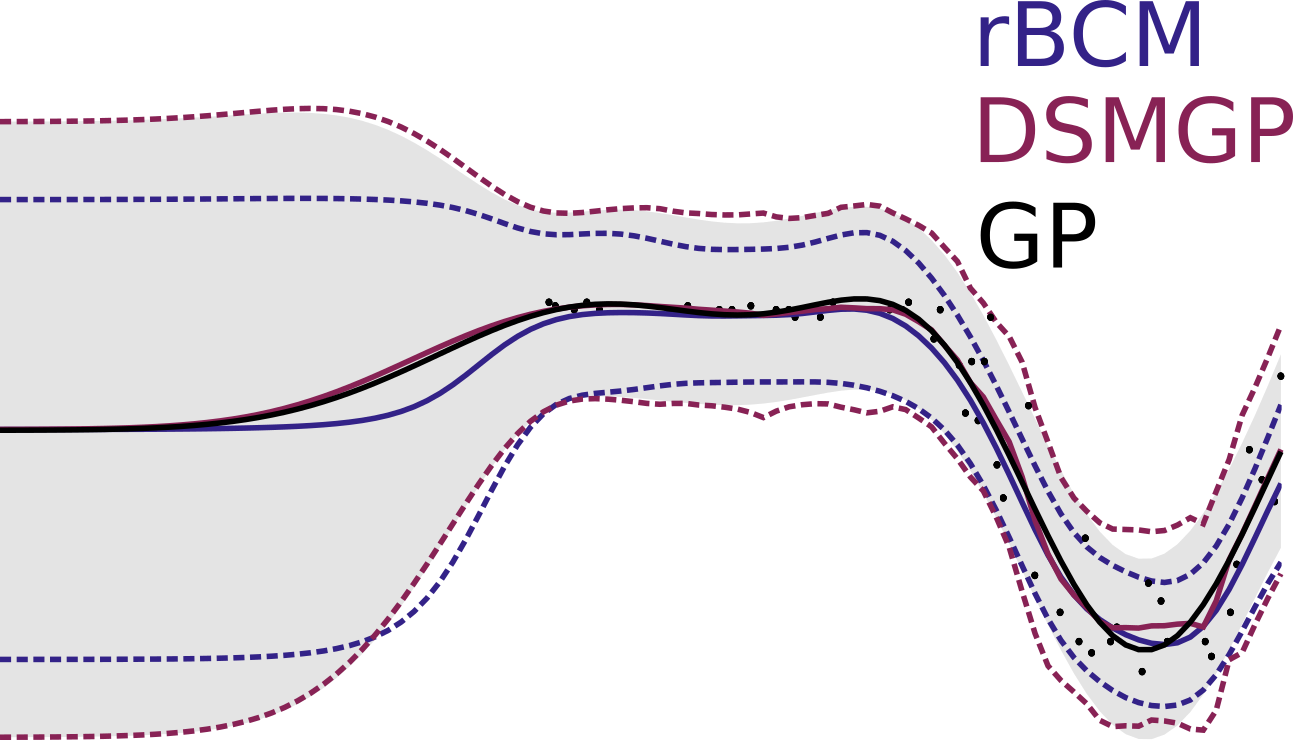
\includegraphics[width=0.5\linewidth]{comparison}
\end{figure}
\end{frame}
